\documentclass{beamer}
\usetheme{Warsaw}
% \usecolortheme{green}

% \definecolor{PRIMARY}{RGB}{0, 100, 0}
% \definecolor{SECONDARY}{RGB}{144,238,144}
% \setbeamercolor{palette primary}{bg=PRIMARY,fg=white}
% \setbeamercolor{palette secondary}{bg=PRIMARY,fg=white}
% \setbeamercolor{palette tertiary}{bg=PRIMARY,fg=white}
% \setbeamercolor{palette quaternary}{bg=PRIMARY,fg=white}
% \setbeamercolor{structure}{fg=PRIMARY} % itemize, enumerate, etc
% \setbeamercolor{section in toc}{fg=PRIMARY} % TOC sections

% % Override palette coloring with secondary
% \setbeamercolor{subsection in head/foot}{bg=SECONDARY,fg=white}

\usepackage{pgfpages}
\setbeameroption{show notes on second screen}

% not included by beamer
\usepackage{multirow}
\usepackage{bm}
\usepackage{pifont}
\newcommand{\cmark}{\ding{51}}
\newcommand{\xmark}{\ding{55}}



\usepackage[style=authoryear]{biblatex}
\bibliography{acl-conf}

\definecolor{darkgreen}{RGB}{0, 100, 0}
\definecolor{navy}{RGB}{0, 0, 128}
\definecolor{darkmagenta}{RGB}{139, 0, 139}
\definecolor{crimson}{RGB}{220, 20, 60}
\definecolor{darkorange}{RGB}{255, 140, 0}

\definecolor{lightyellow}{RGB}{255,255,224}
\definecolor{aliceblue}{RGB}{240,248,255}
\definecolor{grey}{RGB}{192,192,192}



\title[A Local Detection Approach for NER \& MD \hspace{10mm}
		\insertframenumber/\inserttotalframenumber]{
	A Local Detection Approach for \\
	Named Entity Recognition and Mention Detection
}
\author{
	\textbf{Mingbin Xu} \\
	% \vspace{1cm}
	% {\scriptsize Joint work with \\
	% 	\textbf{Hui Jiang} and \textbf{Sedtawut Watcharawittayakul}}
}
\institute{
	Joint work with \textbf{H. Jiang} and \textbf{S. Watcharawittayakul}\\[2ex]

	Lassonade School of Engineering,
	York University,
	Canada

	\begin{figure}
	 	\centering
	  	
\includegraphics[width=4.0cm]{logo}\\
	\end{figure}
}
\date{\small ACL2017}
\begin{document}

\begin{frame}
\titlepage
\end{frame}

\begin{frame}
\frametitle{Outline}
\tableofcontents
\note{
	Good morning. \\
	My name is Mingbin. I am from York University. \\
	This presentation is to report the paper \textsc{
		A Local Detection Approach for Named Entity Recogntion and Mention Detection
	}
}
\end{frame}


\section{Introduction}

\subsection{Task Definition}

\begin{frame}
\frametitle{Entity Discovery}
\begin{definition}
	A sub-task of information extraction that \textcolor{red}{\textbf{finds}} and \textcolor{red}{\textbf{classifies}} entities in text.
\end{definition}
\begin{example}[CoNLL2003 annotation]
	\textcolor{darkorange}{$[Hinton]_{PER}$}, 
	a professor of \textcolor{navy}{$[University\ of\ Toronto]_{ORG}$}, 
	spends several months in \textcolor{navy}{$[Google]_{ORG}$}'s 
	\textcolor{darkgreen}{$[Mountain\ View]_{LOC}$} office every year.
\end{example}
\begin{columns}
	\column{0.5 \textwidth}
	\column{0.5 \textwidth}
	\begin{description}
		\setlength\itemsep{0.05em}
		\small
		\item[\textcolor{darkorange}{PER}] Person
		\item[\textcolor{darkgreen}{LOC}] Location
		\item[\textcolor{navy}{ORG}] Organization
		\item[\textcolor{darkmagenta}{MISC}] Miscellaneous
	\end{description}
\end{columns}
\note{
	NER \& MD sometimes is called entity discovery.\\
	It is a sub-task of information retrieval that finds and classifies entities in text.\\
	For example, in this sentence (read slides),\\
	{ 	\small
		Hinton, a professor of UofT, spends several months in Google's Mountain View office every year.\\
	}
	we want to tell 
	Hinton is a PER, 
	Google is an ORG, and
	Mountain View is a LOC.
}
\end{frame}

\begin{frame}
\frametitle{Entity Discovery}
\begin{definition}
	A sub-task of information extraction that \textcolor{red}{\textbf{finds}} and \textcolor{red}{\textbf{classifies}} entities in text.
\end{definition}
\begin{example}[KBP EDL annotation]
	\textcolor{darkorange}{$[Hinton]_{\textit{PER-NAM}}$}, 
	a \textcolor{darkorange}{$[professor]_{\textit{PER-NOM}}$} of \textcolor{navy}{$[University\ of\ \textcolor{darkmagenta}{[Toronto]_{\textit{GPE-NAM}}}]_{\textit{ORG-NAM}}$}, 
	spends several months in \textcolor{navy}{$[Google]_{\textit{ORG-NAM}}$}'s 
	\textcolor{darkgreen}{$[Mountain\ View]_{\textit{LOC-NAM}}$} office every year.
\end{example}
\begin{columns}
	\column{0.3 \textwidth}
	\column{0.7 \textwidth}
	\begin{description}
		\scriptsize
		\setlength\itemsep{0.02em}
		\small
		\item[\textcolor{darkorange}{PER-\{NAME, NOMINAL\}}] Person
		\item[\textcolor{darkgreen}{LOC-\{NAME, NOMINAL\}}] Location
		\item[\textcolor{navy}{ORG-\{NAME, NOMINAL\}}] Organization
		\item[\textcolor{darkmagenta}{GPE-\{NAME, NOMINAL\}}] Geo-Political Entity
		\item[\textcolor{crimson}{FAC-\{NAME, NOMINAL\}}] Facility
	\end{description}
\end{columns}
\note{
	Some task is more difficult. \\
	We may need to detect nested mentions, 
	e.g. Toronto is embeded in UofT. 
	We need to find out Toronto is GPE and UofT is ORG.\\
	We may also need to detect nominal mentions,
	e.g. We need to know ``professor'' refers to a person in real world.
}
\end{frame}

\subsection{Review}

\begin{frame}
\frametitle{Review}
\begin{figure}
	\centering
	\resizebox{0.7 \textwidth}{!}{
		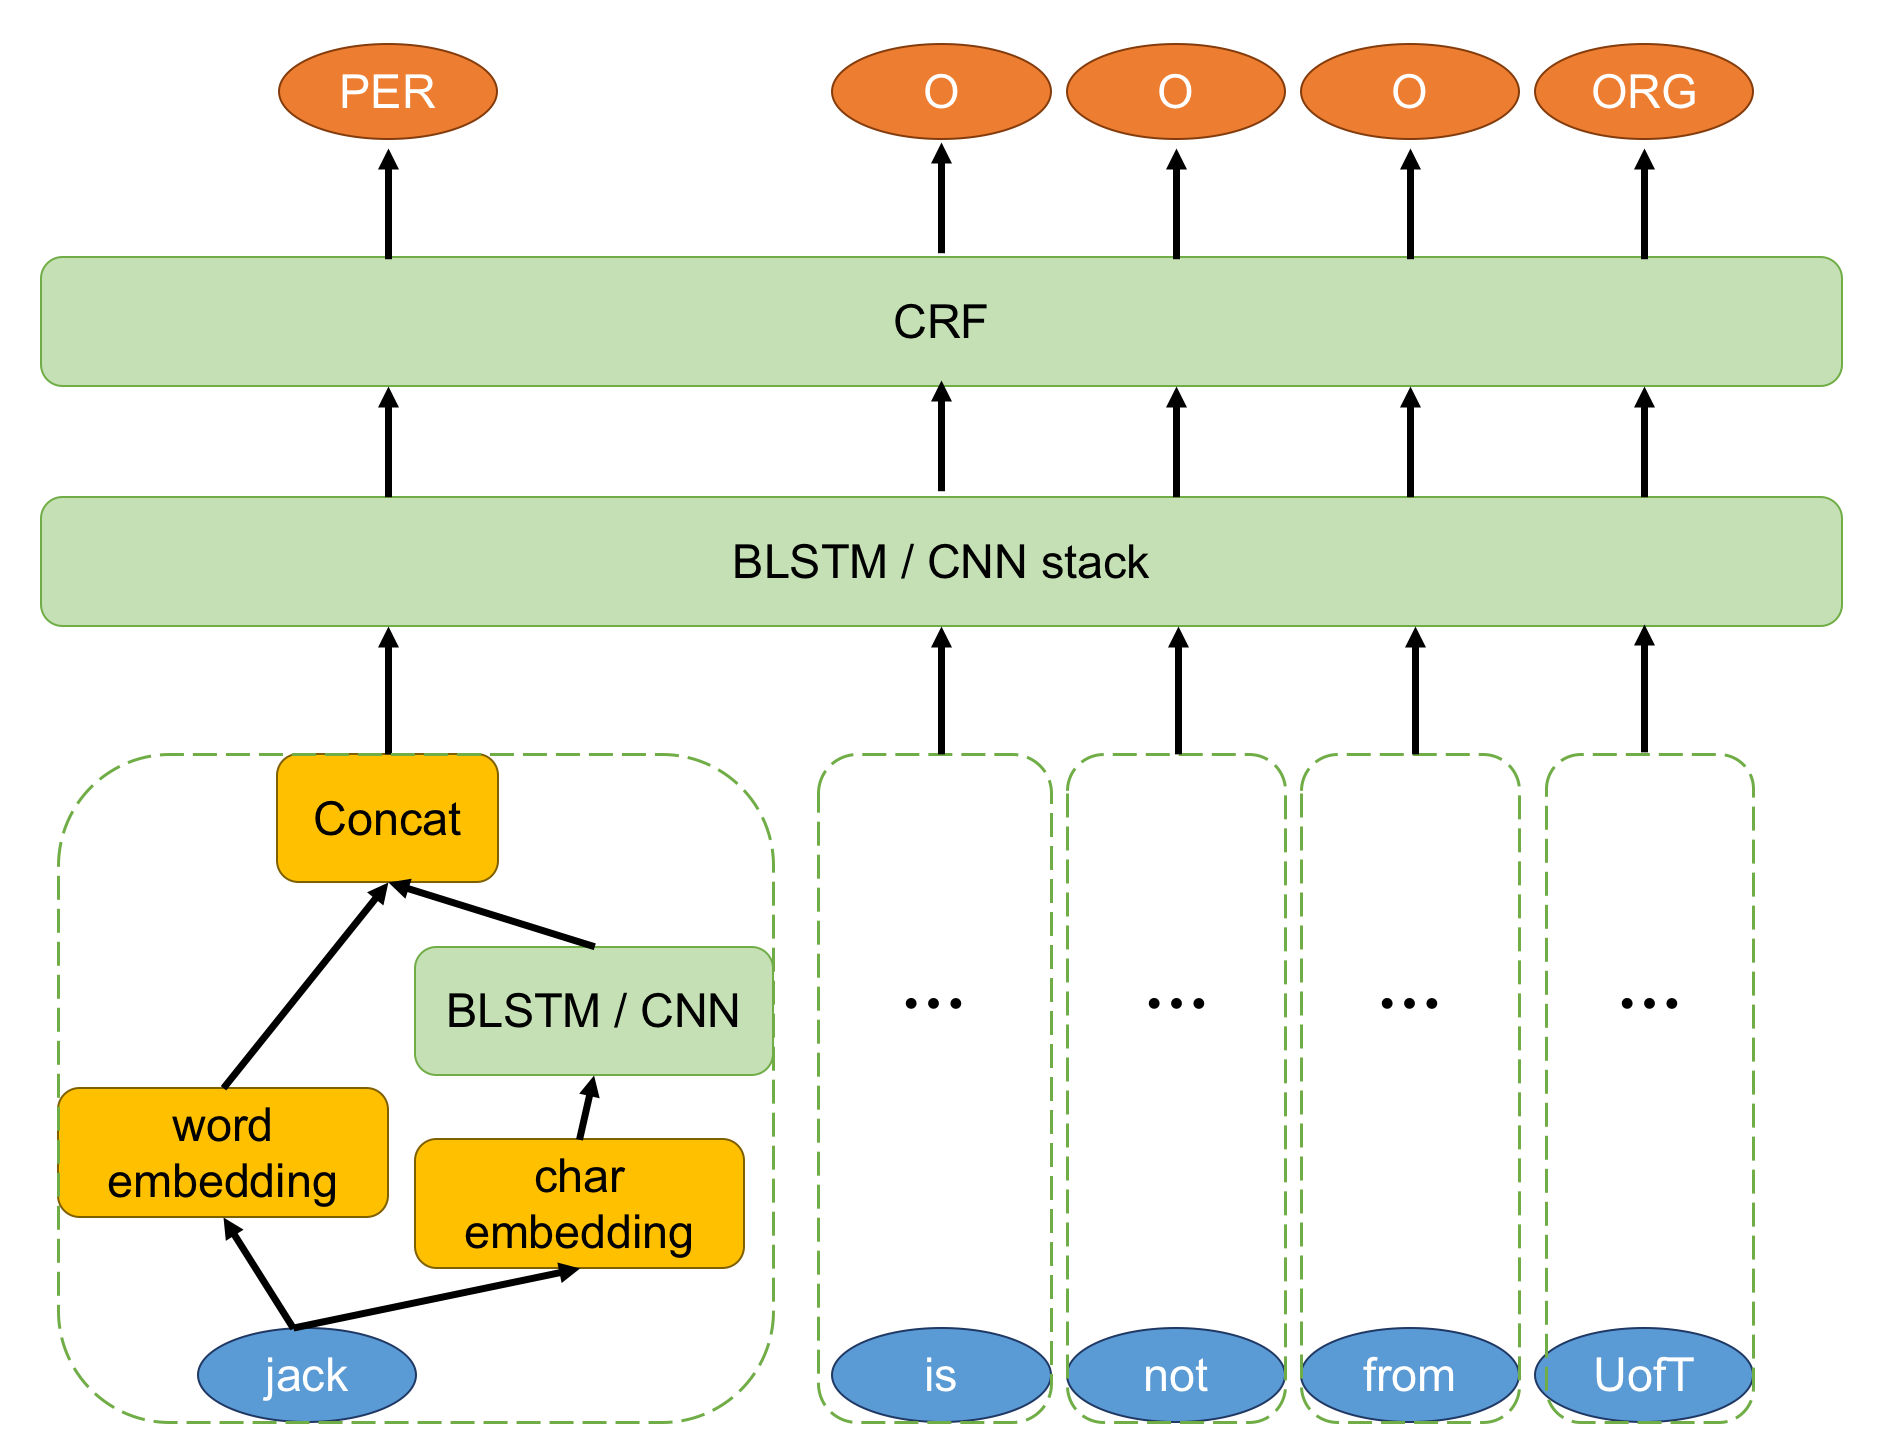
\includegraphics{popular-ner}
	}
	\caption{\scriptsize Illustration of popular neuro-NER models}
\end{figure}
\note{
	A common solution to this problem is sequence labeling.\\
	Each word in a sentence is modeled by word embedding and either CNN or LSTM.\\
	The sentence is modeled by either CNN or LSTM, and decoded by CRF.\\
}
\end{frame}



\section{Preliminary}

\subsection{Fixed-size Ordinally Forgetting Encoding}

\begin{frame}
\frametitle{Fixed-size Ordinally Forgetting Encoding}
\begin{definition}[FOFE]
	\begin{itemize}
	\item $S = w_1, w_2, ..., w_n$ is a sequence of any discrete symbols;
	\item $w_i$ is represented as $\bm{e_i}$ in 1-hot representation;
	\item the encoding of a partial sequence up to the $t$-th word is recursively defined as \parencite{zhang2015fixed}:
	\begin{equation}
		\nonumber
		\bm{z_t}=
		\begin{cases}
		\bm{0}, & \text{if}\ t = 0 \\
		\alpha \cdot \bm{z_{t - 1}} + \bm{e_t}, & \text{otherwise}
		\end{cases}  \label{eq-fofe-def}
	\end{equation}
	\item $\alpha \in (0, 1)$ and $t \in \{{\mathbb Z}|1 \le x \le n\}$
	\end{itemize}
\end{definition}
\note{
	Instead of CNN and LSTM, we adpots another sequence modeling method. \\
	It's \textsc{Fixed-size Orinally Forgetting Encoding}, or FOFE. \\
	Let's say we have a sequence of $n$ symbols, $w1, w2, ..., w_n$. \\
	Each symbol is represented in a 1-hot vector. \\
	The encoding of a partial sequence up to the current symbol is the partial encoding up to the previous symbol plus the 1-hot vector of the current symbol.\\
	$\alpha$ is called forgetting factor. It's usually picked between 0 and 1.
}
\end{frame}


\begin{frame}
\frametitle{Fixed-size Ordinally Forgetting Encoding}
\begin{alertblock}{}
	Any \textcolor{red}{\textbf{variable length}} sequence is encoded into a \textcolor{red}{\textbf{fixed-size}} vector.
\end{alertblock}
\begin{columns}
	\column{0.28 \textwidth}
	\begin{table}
		\centering
		\resizebox{\linewidth}{!}{
		\begin{tabular}{|c|c|}
			\hline
			WORD & 1-HOT \\
			\hline\hline
			$w_0$ & $1000000$ \\
			$w_1$ & $0100000$ \\
			$w_2$ & $0010000$ \\
			$w_3$ & $0001000$ \\
			$w_4$ & $0000100$ \\
			$w_5$ & $0000010$ \\
			$w_6$ & $0000001$ \\
			\hline
		\end{tabular}}
		\caption{\scriptsize Vocab of size 7}
	\end{table}
	\column{0.77 \textwidth}
	\begin{table}
		\centering
		\resizebox{\linewidth}{!}{
		\begin{tabular}{|l|l|}
			\hline
			PARTIAL SEQUENCE & FOFE \\
			\hline\hline
			$w_6$ & $0, 0, 0, 0, 0, 0, 1$ \\
			$w_6, w_4$ & $0, 0, 0, 0, 1, 0, \alpha$ \\
			$w_6, w_4, w_5$ & $0, 0, 0, 0, \alpha, 1, \alpha^2$ \\
			$w_6, w_4, w_5, w_0$ & $1, 0, 0, 0, \alpha^2, \alpha, \alpha^3$ \\
			$w_6, w_4, w_5, w_0, w_5$ & $\alpha, 0, 0, 0, \alpha^3, 1 + \alpha^2, \alpha^4$ \\
			$w_6, w_4, w_5, w_0, w_5, w_4$ & $\alpha^2, 0, 0, 0, 1 + \alpha^4, \alpha + \alpha^3, \alpha^5$ \\
			\hline
		\end{tabular}}
		\caption{\scriptsize Partial encoding of $w_6, w_4, w_5, w_0, w_5, w_4$}
	\end{table}
\end{columns}
\note{
	Since the encoding is weighted sum of each symbol, its size depends on vocabulory size only.\\
	It is able to encode any sequence into a fixed-size vector.
}
\end{frame}

\subsection{Uniqueness of FOFE}

\begin{frame}
\frametitle{Uniqueness of FOFE}
\begin{theorem}
	If the forgetting factor $\alpha$ satisfies $0 < \alpha \leq 0.5$, 
	FOFE is unique for any countable vocabulary $V$ and any finite value $T$.
\end{theorem}
\begin{theorem}
	For $0.5 < \alpha < 1 $, given any finite value $T$ and any countable vocabulary $V$,
	FOFE is almost unique everywhere, except only a finite set of countable choices of $\alpha$.
\end{theorem}
% \begin{proof}
% 	% \begin{enumerate}[i]
% 	% \item 
% 	(1) $\sum\limits_{n=0}^{\infty} \alpha^n \le 1$; \\
% 	% \item 
% 	(2) $c_0 \times \alpha^0 + c_1 \times \alpha^1 + ... + c_n \times \alpha^n = 0$, $c_i \in \{-1, 0, 1\}$
% 	% \end{enumerate}
% \end{proof}
\note{
	FOFE has a very nice uniqueness property. \\
	(READ SLIDES) \\
	{	\small
		if $\alpha$ is between 0 and 0.5, FOFE is unique for any countable vocabulary V and any finite value T. \\
		if $\alpha$ is between 0.5 and 1, given any finite value T and countable vocabulary V, FOFE is almost unique, except a finite set of countable choices of $\alpha$.\\
	}
	Simply put, FOFE is a lossless fixed-size prepresentation for sequence modeling.
}
\end{frame}


\subsection{Efficiency of FOFE}
\begin{frame}
\frametitle{Computational Efficiency of FOFE}
% \begin{columns}
	% \column{0.51 \textwidth}
	\begin{block}{LSTM}
		One step at a time; each involves 4 matrix multications.
		\begin{align*}
		x & = oneHot([w_1, w_2, ..., w_n]) \times W_{embed}\\
		C_t, h_t & = LSTM(x_t, C_{t-1}, h_{t_1})\\
		enc([w_1, ..., w_n]) & = C_n
		\end{align*}
		% \begin{equation}
		% 	\begin{aligned}
		% 		i_t = \sigma(W_i \cdot [h_{t-1}, x_t] + b_i) \\
		% 		f_t = \sigma(W_f \cdot [h_{t-1}, x_t] + b_f) \\
		% 		f_t = \sigma(W_o \cdot [h_{t-1}, x_t] + b_o) \\
		% 		{\tilde{C}}_t = \sigma(W_c \cdot [h_{t-1}, x_t] + b_c) \\
		% 		C_t = i_t \times {\tilde{C}}_t + f_t \times C_{t-1} \\
		% 		h_t = o_t \times \sigma(C_t)
		% 	\end{aligned}
		% \end{equation}
	\end{block}
	% \column{0.51 \textwidth}
	\begin{block}{FOFE}
		A single matrix multiplication leads to the final encoding.
		\begin{align*}
			alpha & = [\alpha^{n-1}, \alpha^{n-2}, ... , \alpha, 1] \\
			enc([w_1, ..., w_n])
			& =
				\textbf{\textcolor{red}{(}} alpha
				\times oneHot([w_1, w_2, ..., w_n])
				\textbf{\textcolor{red}{)}} \times W_{embed} \\
			& =
				alpha \times \textbf{\textcolor{red}{(}}
				oneHot([w_1, w_2, ..., w_n]) \times W_{embed}
				\textbf{\textcolor{red}{)}}
		\end{align*}
	\end{block}
% \end{columns}
\note{
	FOFE is significantly faster than LSTM.\\
	e.g. In LSTM, we first get the embedding by of each word. It's conceptually a matrix multiplication. It is implememted as table lookup. Then, the encoding at each postion must be computed step by step. Each step consists of 4 matrix multiplications. \\
	FOFE conceptually a vector of geometric series times the matrix of one-hot vectors. 
	Similarly, word embedding is used to reduce dimensions. 
	Because of associativity of matrix multipliation, we can do table lookup first to get a much smaller matrix. A single matrix multiplicatio leads to the final encoding of the sentence. 
}
\end{frame}


\begin{frame}
\frametitle{Universial Framework for NLP}
\begin{figure}
	\centering
	\resizebox{0.56 \textwidth}{!}{
		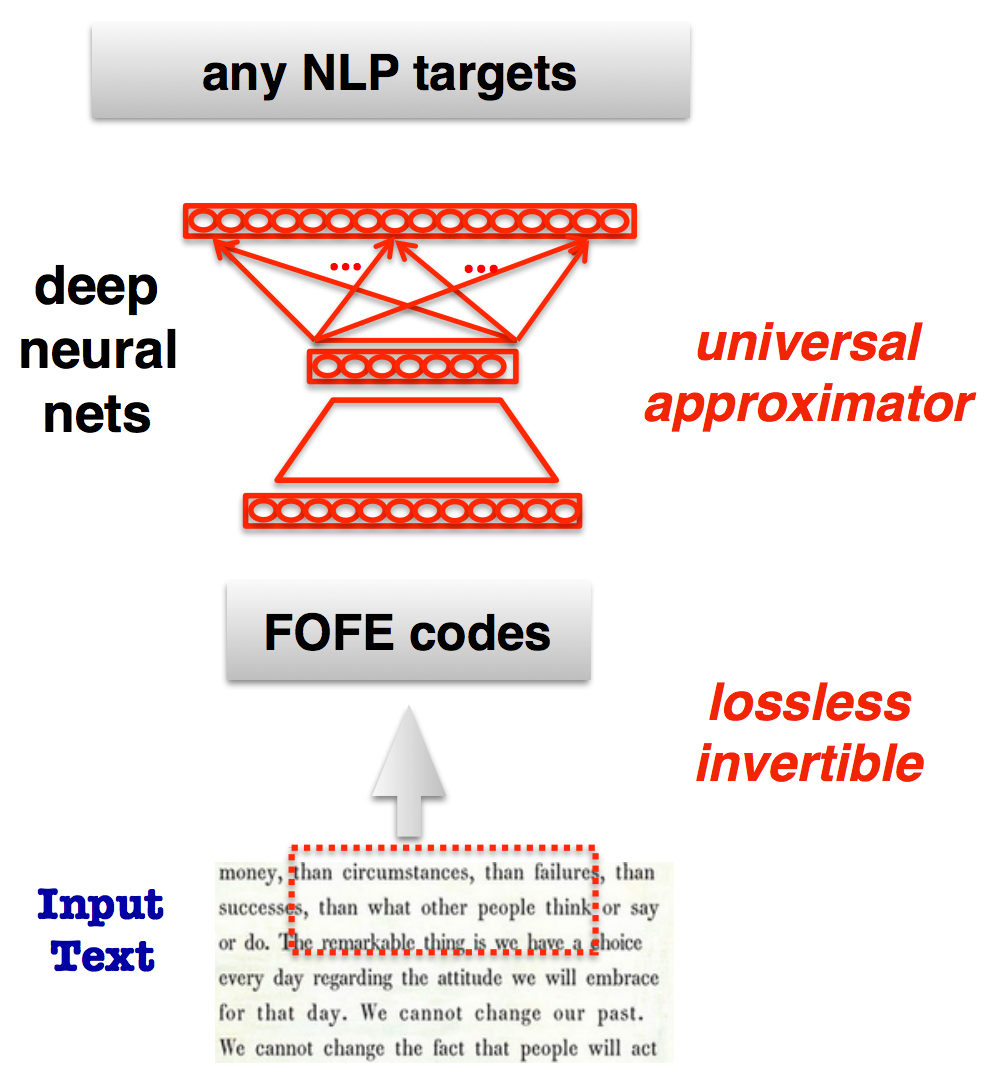
\includegraphics{fofe-ffnn-nlp}
	}
	\caption{\scriptsize FOFE-FFNN for NLP}
\end{figure}
\note{
	Because FOFE is lossless fixed-size representation and FFNN is a universial approximator,\\
	FOFE plus FFNN serves as a universail framework for NLP.\\
}
\end{frame}


% TODO: add general architecture of FOFE4NLP


\section{Local Detection Algorithm}

\subsection{Algorithm}

\begin{frame}
\frametitle{Local Detection}
\begin{block}{Intuition}
	\begin{itemize}
	\item People rarely conduct a global decoding over the entire sentence to pinpoint entities.
	\item The key to accurate local detection is to have full access to
		\textbf{\textcolor{red}{the fragment itself}}, and
		\textbf{\textcolor{red}{its contextual information}}.
	\item FOFE is a \textbf{\textcolor{red}{lossless}} representation of \textbf{\textcolor{red}{fixed length}}.
	\end{itemize}
\end{block}
\begin{example}
    \begin{itemize}
    \item \textbf{\textcolor{navy}{$[S.E.C.]_{ORG}$}} chief 
            \textbf{\textcolor{darkorange}{$[Mary\ Shapiro]_{PER}$}} left 
            \textbf{\textcolor{darkgreen}{$[Washington]_{LOC}$}} in December. \\
    \item Do the entity types of ``S.E.C'' and ``Washington'' matter? How about:
    \textbf{Our} chief Mary Shapiro left \textbf{us} in December?
    \end{itemize}
\end{example}
\note{
	Here's our \textsc{Local Detection} algorithm.\\
	The intution behind this idea is that: \\
	(read slides)\\
	{\small
		People rarely conduct a global decoding over the entire sentence to pinpoint entities.\\
		he key to accurate local detection is to have full access to the fragment itself, and its contextual information.\\
		We picked FOFE as our method of modeling these two pieces because FOFE is a lossless representation of fixed length.\\
	}
	Let's say we're interested in the text fragment May Shapiro in this sentence.\\
	As long as we know it is a cheif and it can performs an action of ``left'', we can tell it's a person. Whether S.E.C is an ORG or not and whether Washington is a LOC or not do not affect our decision.
}
\end{frame}

\begin{frame}
\begin{block}{Algorithm}
	\begin{overprint}
	\onslide<1>
		Our methods treats the \textcolor{red}{\textbf{whole sentence}} as context to make a local decision for each text fragment.
	\onslide<2>
		\begin{itemize}
		\item Extract features from \textbf{\textcolor{red}{each segment}} and send to FFNN.
		\item Remove overlapping / inconsistent labels.
		\end{itemize}
	\end{overprint}
\end{block}
\begin{figure}
	\centering
	\resizebox{0.88 \textwidth}{!}{
		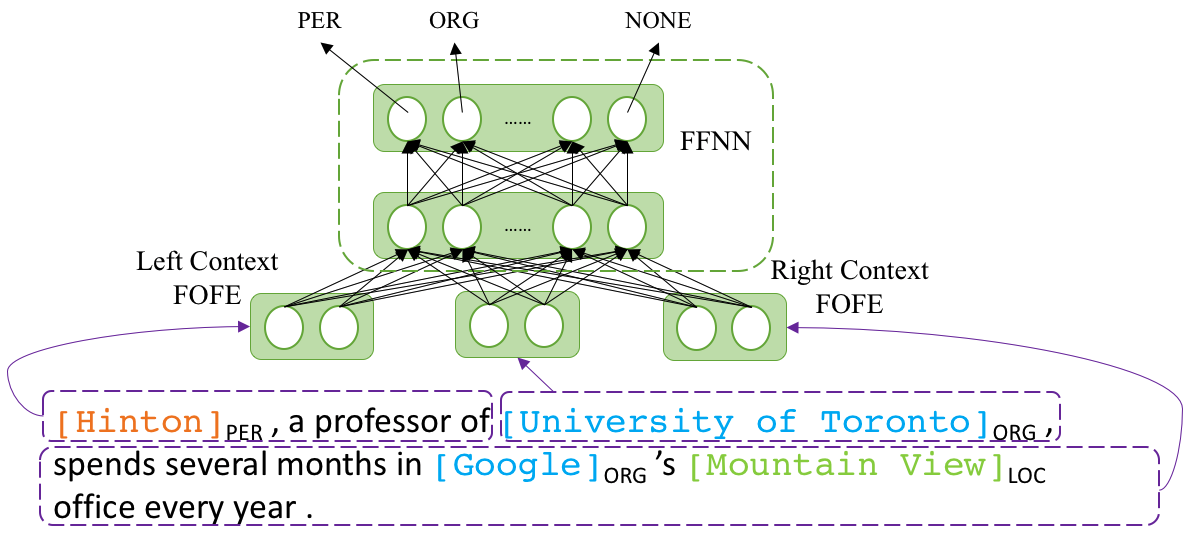
\includegraphics{algo}
	}
	\caption{\scriptsize Illustration of local detection}
\end{figure}
\note{
	Unlike previous local detection approach, ours \textsc{Local Detection} approach treat the entire sentence as context. \\
	The local decision is made based on global information.

	\textcolor{red}{\textbf{(Next)}}
	
	Our \textsc{Local Detection} approach extract features from each segment and sends them to an FFNN.\\
	Let's say the text fragment we're interested in is ``UofT''.\\
	It divides the sentence into 3 disjoint sub-sequence.\\
	Everything to the left of UofT is called left context. \\
	Everything to the right of UofT is called right context. \\
	Becuase these 3 pieces are sequences of words. They can be easily modeled by FOFE.\\
	Because FOFE is fixed-size, we pick FFNN as our classifier. \\
}
\end{frame}


\subsection{Feature Extraction}

\begin{frame}
\frametitle{Feature Extraction}
\begin{block}{Feature Extraction}
	\footnotesize
	\begin{table}
		%\small
		\centering
		\begin{tabular}{|r|p{0.36\textwidth}|p{0.44\textwidth}|}
		% \resizebox{0.96 \textwidth}{!}{
		% \begin{tabular}{r|l|l}
		\hline
		& text segment & context \\
		\hline \hline
		\multirow{4}{*}{\shortstack{word\\level}}
		& \multirow{2}{*}{\textcolor<2>{red}{BoW}} 
		&   \textcolor<5>{red}{left FOFE excl. text fragment} \\ \cline{3-3}
		& & \textcolor<5>{red}{right FOFE excl. text fragment} \\ \cline{2-3}
		& \multicolumn{2}{c|}{\textcolor<6>{red}{left FOFE incl. text fragment}}\\ \cline{2-3}
		& \multicolumn{2}{c|}{\textcolor<7>{red}{right FOFE incl. text fragment}} \\
		\hline
		\multirow{2}{*}{\shortstack{char\\level}}
		& \textcolor<4>{red}{Char CNN \parencite{kim2015character}} & \multirow{2}{*}{N/A} \\
		& \textcolor<3>{red}{Char FOFE} & \\
		\hline
		\end{tabular}%}
	\end{table}
\end{block}
\begin{example}[\footnotesize examining `Mary Shapiro']
	\footnotesize
	\begin{overprint}
		\centering
		\onslide<1>
			\textbf{\textcolor{navy}{$[S.E.C.]_{ORG}$}} chief
		    \textbf{\textcolor{darkorange}{$[Mary\ Shapiro]_{PER}$}}
		    left \textbf{\textcolor{darkgreen}{$[Washington]_{LOC}$}} in December.
		\onslide<2-4>
			\textbf{\textcolor{navy}{$[S.E.C.]_{ORG}$}} chief
    		\colorbox{grey}{\textbf{\textcolor{darkorange}{$[Mary\ Shapiro]_{PER}$}}}
    		left \textbf{\textcolor{darkgreen}{$[Washington]_{LOC}$}} in December.
		\onslide<5>
			\colorbox{grey}{\textbf{\textcolor{navy}{$[S.E.C.]_{ORG}$}} chief}
		    \textbf{\textcolor{darkorange}{$[Mary\ Shapiro]_{PER}$}}
		    \colorbox{grey}{left \textbf{\textcolor{darkgreen}{$[Washington]_{LOC}$}} in December.}
		\onslide<6>
			\colorbox{grey}{
				\textbf{\textcolor{navy}{$[S.E.C.]_{ORG}$}} chief
		    	\textbf{\textcolor{darkorange}{$[Mary\ Shapiro]_{PER}$}}
		    }
		    left \textbf{\textcolor{darkgreen}{$[Washington]_{LOC}$}} in December.
		\onslide<7>
			\textbf{\textcolor{navy}{$[S.E.C.]_{ORG}$}} chief
			\colorbox{grey}{
		    	\textbf{\textcolor{darkorange}{$[Mary\ Shapiro]_{PER}$}}
		    	left \textbf{\textcolor{darkgreen}{$[Washington]_{LOC}$}} in December.
		    }
	\end{overprint}
\end{example}
\note{
	we model the text fragment at word level and character level.\\
	Let's say we're interested in the text fragment ``Mary Shapiro'' in this sentence. 
	\textcolor{red}{\textbf{(Next)}}\\
	The text fragment is first modeled by BoW. 
	\textcolor{red}{\textbf{(Next)}}\\
	At the same time, it can be viewed as a character sequence. So we can construct a bi-directional FOFE to model its internal structure. 
	\textcolor{red}{\textbf{(Next)}}\\
	Similary, we apply character CNN as well. 
	\textcolor{red}{\textbf{(Next)}}\\
	In terms of context feature, we build 2 FOFE represnetation for left context and right context respectively. 
	\textcolor{red}{\textbf{(Next)}}\\
	Finally, in order to emphize the order of words in the text fragment and their relationship to the context, we create 2 more FOFE representation.
	One is from the start of the sentence to the end of the text fragment.
	The other one is from the end ofthe sentence to the start of the text fragment.
}
\end{frame}

% \subsection{2nd-pass Enhancement}

% \begin{frame}
% \frametitle{2nd-pass Enhancement}
% \begin{block}{2nd-pass Trainer}
% 	If we substitute entities in context with general types, the model
% 	\begin{itemize}
% 	\item captures the semantic roles of other entities,
% 	\item filters out unwanted constructs and sparse combinations, and
% 	\item enables longer context expansion.
% 	\end{itemize}
% \end{block}
% \begin{example}[\scriptsize Examining ``University of Toronto'']
% 	\textcolor{darkorange}{{\textless}PER{\textgreater}}, 
% 	a professor of \textcolor{navy}{$[University\ of\ Toronto]_{ORG}$}, 
% 	spends several months in \textcolor{navy}{{\textless}ORG{\textgreater}}'s 
% 	\textcolor{darkgreen}{{\textless}LOC{\textgreater}} office every year.
% \end{example}
% \end{frame}

% \begin{frame}
% \frametitle{2nd-pass Enhancement}
% \begin{figure}
% 	\centering
% 	\resizebox{0.81 \textwidth}{!}{
% 		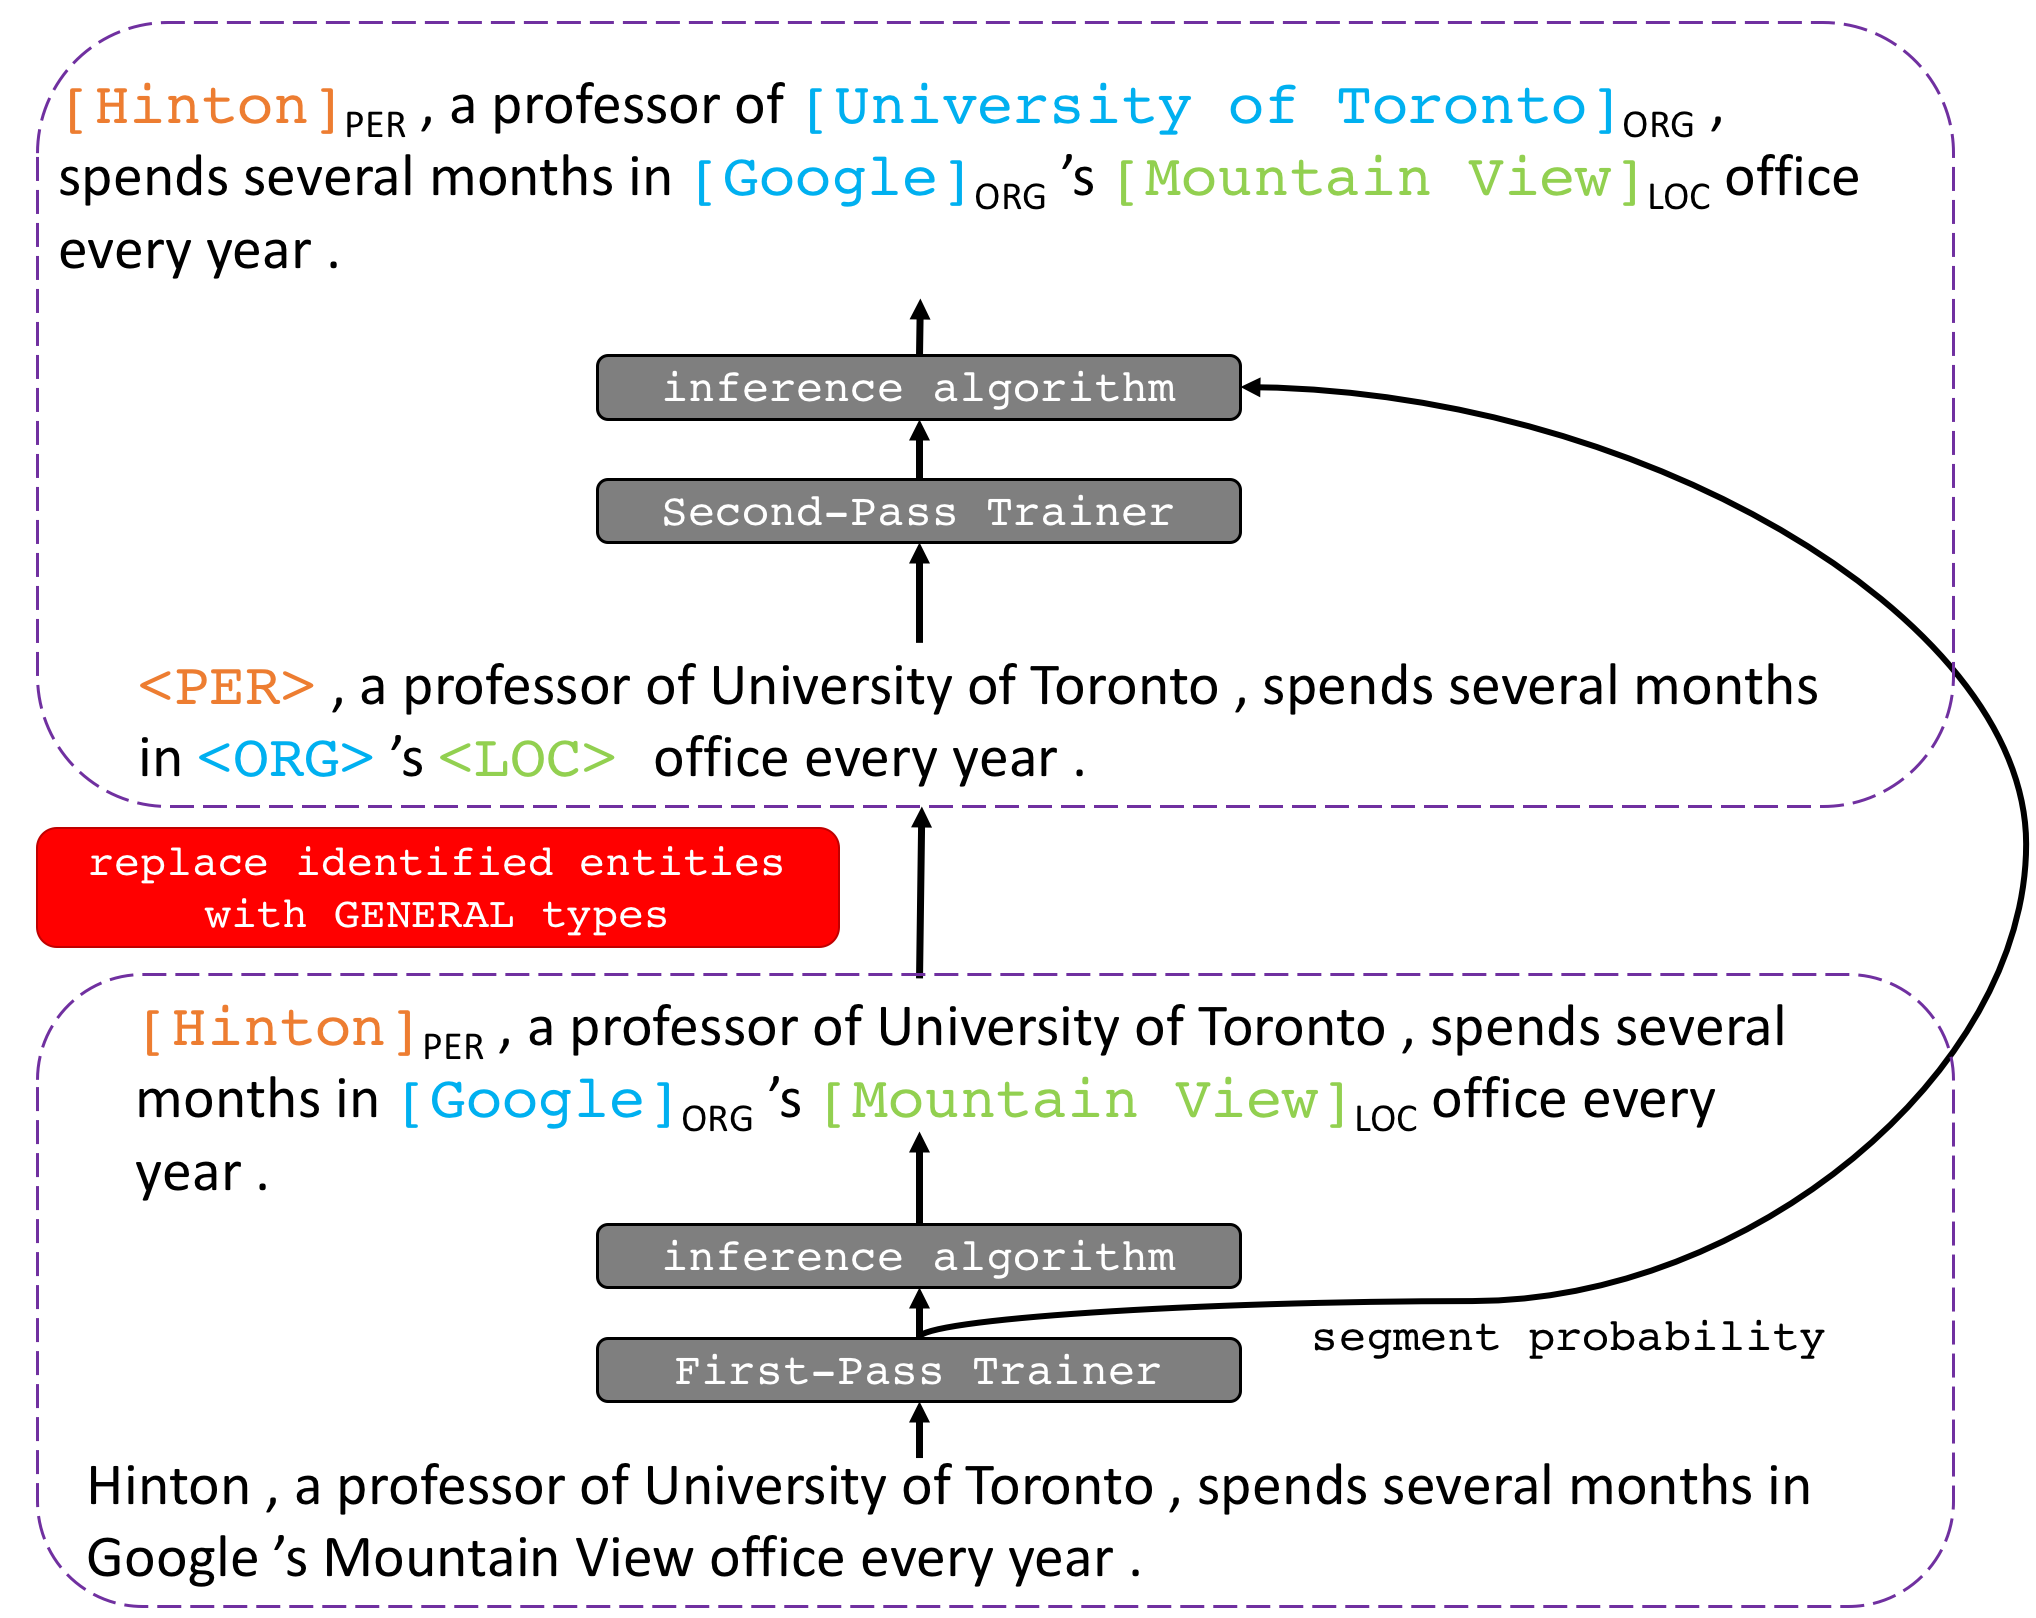
\includegraphics{system}
% 	}
% \end{figure}
% \end{frame}


\subsection{Model Advantage}

\begin{frame}
\frametitle{Model Advantages}
% \small
% \begin{block}{Computational Efficiency}
% 	\begin{itemize}
% 		\item FOFE can be expressed as sparse matrix, i.e. $indices$ \& $values$
% 		\item $fofe(seq) \cdot embed = 
% 				[\alpha^{n-1}, ..., \alpha, 1] \cdot lookup(seq, embed)$
% 	\end{itemize}
% \end{block}
\begin{block}{Data Availability}
	Correct annotation for the entire sentence is NOT a must.
	\begin{itemize}
		\item Data annotated with different standard are more usable.
		\item Wikipedia highlights an entity's first appearance.{\scriptsize\parencite{nothman2013learning}}
	\end{itemize}
\end{block}
\begin{alertblock}{Advantage over Known Methods}
	\begin{itemize}
		\item Nested depth control
		\item Feature-engineering-free
	\end{itemize}
\end{alertblock}
\note{
	Our model has several advantages over existing solutions.\\

	Since it's local detection, correct annotation for the entire sentence is not a must.\\
	As long as one entity is correctly labled, it can be used as a training example. \\
	So, data annotated with different standard are more usable. \\
	Wikipedia highlights an entity's first apperance in an article. This kind of machine-generated data is very accurate locally.

	We assign scores for each text fragment. e.g. if we use the example of UofT, UofT has its own score and Toronto has its own score. \\
	The user detects nested entity. He can easily control whether to keep it or not based on the task definition.\\
	Another benefit is that our word level feature and character feature are derived from data. There is not feature engineering at all.
}
\end{frame}



\section{Experiments} 


\subsection{CoNLL2003}

\begin{frame}
\frametitle{CoNLL2003 Shared Task}
\begin{block}{CoNLL2003 Shared Task}
	\begin{itemize}
	\item newswire from the Reuters RCV1 corpus;
	\item tagged with 4 types of \textbf{\textcolor{red}{non-nested}} named entities: 
			\textcolor{darkorange}{Person (PER)}, 
			\textcolor{navy}{Organization (ORG)},
			\textcolor{darkgreen}{Location (LOC)}, and
			\textcolor{darkmagenta}{Miscellaneous (MISC)}.
	\end{itemize}
\end{block}
\begin{table}
    \centering
    \resizebox{0.9 \textwidth}{!}{
    \begin{tabular}{c|ccc|cccc}
         & Articles & Sentences & Tokens & LOC & MISC & ORG & PER \\
        \hline
        train & 946 & 14,987 & 203,621 & 7,140 & 3,438 & 6,321 & 6,600 \\
        dev & 216 & 3,466 & 51,362 & 1,837 & 922 & 1,341 & 1,842  \\
        test & 231 & 3,684 & 46,435 & 1,668 & 702 & 1,661 & 1,617 
    \end{tabular}}
    \caption{\scriptsize Data distribution of CoNLL2003}
    \label{tbl:conll2003stat}
\end{table}
\note{
	We first evaluate our model on CoNLL2003 shared task. \\
	The task defines 4 non-nested named entities. 
}
\end{frame}

\begin{frame}
\frametitle{Feature Effectiveness}
\begin{table}
	% \scriptsize
	\centering
	% \resizebox{0.93\linewidth}{!}{
	\resizebox{0.98\linewidth}{!}{
	\begin{tabular}{|l|l|l|lll|}
		\hline
		\multicolumn{3}{|c|}{FEATURE} & P & R & F1\\
		\hline\hline
		\multirow{6}{*}{\shortstack{word\\level}} & 
		\multirow{3}{*}{\shortstack[l]{case-\\insensitive}} &
		context FOFE incl. word fragment & 86.64 & 77.04 & 81.56 \\
		& &context FOFE excl. word fragment & 53.98 & 42.17 & \textcolor<2-3>{red}{47.35} \\
		& & BoW of word fragment & 82.92 & 71.85 & \textcolor<2-3>{red}{76.99}  \\ \cline{2-6} 
		& \multirow{3}{*}{\shortstack[l]{case-\\sensitive}} & 
		context FOFE incl. word fragment & 88.88 & 79.83 &84.12  \\
		& &context FOFE excl. word fragment & 50.91 & 42.46 & 46.30  \\
		& & BoW of word fragment & 85.41 & 74.95 & 79.84  \\ \hline
		\multirow{2}{*}{\shortstack{char\\level}} &
		\multicolumn{2}{l|}{Char FOFE of word fragment} & 67.67 & 52.78 & 59.31  \\
		& \multicolumn{2}{l|}{Char CNN of word fragment} & 78.93 & 69.49 & 73.91 \\ \hline
		\multicolumn{3}{|l|}{all case-insensitive features} &  90.11 & 82.75 &  86.28  \\ 
		\multicolumn{3}{|l|}{all case-sensitive features} & 90.26 & 86.63 & 88.41 \\ 
		\multicolumn{3}{|l|}{all word-level features} & 92.03 & 86.08 & \textcolor<3>{red}{88.96} \\ \hline
		\multicolumn{3}{|l|}{all word-level \& Char FOFE features} & 91.68 &  88.54 & \textcolor<4>{red}{\bf 90.08} \\
		\multicolumn{3}{|l|}{all word-level \& Char CNN features} & 91.80 & 88.58 & \textcolor<4>{red}{\bf 90.16} \\ \hline
		\multicolumn{3}{|l|}{all word-level \& all char-level features}  & 93.29 &  88.27 &  \bf 90.71  \\
		% \multicolumn{3}{|l|}{all features + {\bf dev set} + 5-fold cross-validation} & 92.58 &  89.31 &  \bf 90.92  \\
		% \multicolumn{3}{|l|}{all features + {\bf 2nd-pass}} & 92.13 &  89.61 &  \bf 90.85  \\
		% \multicolumn{3}{|l|}{all features + {\bf 2nd-pass} + {\bf dev set} + 5-fold cross-validation} & 92.62 &  89.77 &  \bf 91.17 \\
		\hline
	\end{tabular}}
	\caption{\scriptsize Effect of various FOFE feature combinations on the CoNLL2003 test data.}
	\label{tbl:feat-cmp:CoNLL03}
\end{table}
% \pause
%   \vskip-3cm
%   \begin{block}{The Overlay Block}
%     Block Text
%   \end{block}
\note{
	Let's look at the effectivenes of various features. 
	\textcolor{red}{\textbf{(Next)}}\\
	From line2, we can see that the context along does much better than random guess. It proves that context is a deciding factor.\\
	From line3, we can see that the text fragment alone is not strong enough. It's ambiguous. 
	\textcolor{red}{\textbf{(Next)}}\\
	From line11, we can see that when we combined all word level features of text fragment and context, it allows us to make accurate local decision. 
	\textcolor{red}{\textbf{(Next)}}\\
	Line 12 includes character FOFE. Line 13 includes character. FOFE is competitive to CNN when modeling the internal structure of the text fragment.
}
\end{frame}

\begin{frame}
\frametitle{Comparison between Neural Network Models}
\begin{table}
	\centering
	\resizebox{\linewidth}{!}{
	\begin{tabular}{|l|lllll|l|}
		\hline
		 algorithm & word & char & gaz & cap & pos & F1 \\
		\hline\hline
		 {CNN-BLSTM-CRF} \parencite{collobert2011natural} & \cmark & \xmark & \cmark & \cmark & \xmark & 89.59  \\
		 {BLSTM-CRF} \parencite{huang2015bidirectional}  &\cmark & \cmark & \cmark & \cmark & \cmark & 90.10 \\
		 {BLSTM-CRF} \parencite{rondeau2016lstm}  & \cmark & \xmark & \cmark & \cmark & \cmark & 89.28 \\
		{BLSTM-CRF, char-CNN} \parencite{chiu2016named}  & \cmark & \cmark & \cmark & \xmark & \xmark & {\bf 91.62} \\
		{Stack-LSTM-CRF, char-LSTM} \parencite{lample2016neural}  & \cmark & \cmark & \xmark & \xmark & \xmark & {\bf 90.94} \\
		\hline \hline
		{\bf FOFE-NER} (single) & \cmark & \cmark & \xmark & \xmark & \xmark & {\bf 90.71} \\
		% {\bf FOFE-NER} (single) + 2nd-pass  & \cmark & \cmark & \xmark & \xmark & \xmark & {\bf 90.85} \\
		{\bf FOFE-NER} (ensemble) + dev  & \cmark & \cmark & \xmark & \xmark & \xmark & {\bf 90.92} \\
		% {\bf FOFE-NER} (ensemble) + dev + 2nd-pass  & \cmark & \cmark & \xmark & \xmark & \xmark & {\bf 91.17} \\
		\hline
	\end{tabular}}
	\caption{\scriptsize Performance ($F_1$ score) comparison among various neural models reported on the CoNLL dataset, and the different features used in these methods.}
	\label{tbl:nn-cmp:CoNLL03}
\end{table}
\note{
	In this table, we comare our result with other neural network models.\\
	Except the model in line 5, all other methods involves heavy feature engineering or make use of external knowledge.\\
	However, the model in line 5 is much more computationally expensive than ours.
}
\end{frame}




\subsection{EDL in KBP2015}
\label{subsec:kbp2015}

\begin{frame}
\frametitle{EDL in KBP2015}
\begin{block}{EDL Track in KBP2015 \parencite{kbpoverview2015}}
\begin{itemize}
	\item Requires to identify entities \textbf{\textcolor{red}{(including nested entities)}} from English, Chinese and Spanish documents.
	\item 5 entity types are defined, i.e. Person (PER), Geo-political Entity (GPE), Organization (ORG), Location (LOC) and Facility (FAC).
	\item Documents are related but \textbf{\textcolor{red}{non-parallel}} across languages. 
\end{itemize}
\end{block}
\begin{table}
	%\resizebox{\linewidth}{!}{
		\centering
		\begin{tabular}{|l|c|c|c|c|}
			\hline
			& English & Chinese & Spanish & ALL \\
			\hline
			Train & 168 & 147 & 129 & 444 \\
			Eval & 167 & 167 & 166 & 500 \\
			\hline
		\end{tabular}%}
	\caption{\scriptsize Number of Documents in KBP2015}
	\label{tbl:kbp2015stat}
\end{table}
\note{
	We further evaluate our model using the EDL track in KBP2015. \\
	The contest is trilingual.\\
	Documents are related but not parallel.
}
\end{frame}

\begin{frame}
\frametitle{EDL in KBP2015}
\begin{table}
	\resizebox{\linewidth}{!}{
	\centering
	\begin{tabular}{|l|lll|lll|}
		\hline
		\ & \multicolumn{3}{c|}{2015 track best} & \multicolumn{3}{c|}{FOFE-NER} \\
		\cline{2-7}
		\ & $P$ & $R$ & $F_{1}$ & $P$ & $R$ & $F_{1}$ \\
		\hline \hline
		Trilingual & 75.9 & 69.3 & 72.4 & 78.3 & 69.9 & \bf 73.9 \\
		English & 79.2 & 66.7 & \bf 72.4 & 77.1 & 67.8 & 72.2 \\
		Chinese & 79.2 & 74.8 & \bf 76.9 & 79.3 & 71.7 & 75.3 \\
		Spanish & 78.4 & 72.2 & 75.2 & 79.9 & 71.8 & \bf 75.6 \\
		\hline
	\end{tabular}}
	\caption{\scriptsize Entity Discovery Performance of our method on the KBP2015 EDL evaluation data, with comparison to the best systems in KBP2015 official evaluation.}
	\label{tbl:kbp2015cmp}
\end{table}
\note{
	On the left hand side of the table, we have the perfrmance of the track best. \\
	Ours is on the right hand side.\\
	Our model performs similarly to the best in English and CHinese, and surpasses the best in Spanish and the overall performance. \\

}
\end{frame}


\subsection{EDL in KBP2016}

\begin{frame}
\frametitle{EDL in KBP2016}
\begin{block}{EDL Track in KBP2016 \parencite{kbpoverview2016}}
\begin{itemize}
	\item The task is extended to detect \textbf{nominal mentions} of all 5 entity typess. 
	\item We treat nominal mention types as some extra entity types and detect them along with named entities.  
\end{itemize}
\end{block}
\begin{example}
	\textcolor{darkorange}{$[Hinton]_{\textit{PER-NAM}}$}, 
	a \colorbox{lightyellow}{\textcolor{darkorange}{$[professor]_{\textit{PER-NOM}}$}} of \textcolor{navy}{$[University\ of\ \textcolor{darkmagenta}{[Toronto]_{\textit{GPE-NAM}}}]_{\textit{ORG-NAM}}$}, 
	spends several months in \textcolor{navy}{$[Google]_{\textit{ORG-NAM}}$}'s 
	\textcolor{darkgreen}{$[Mountain\ View]_{\textit{LOC-NAM}}$} office every year.
\end{example}
\note{
	We participated the EDL track of KBP2016.\\
	The task is much harder in the sense that the particpants were asked to annotate nominal mentions.
}
\end{frame}

\begin{frame}
\frametitle{Training Data for KBP2016}
\begin{block}{Training and evaluation data in KBP2015}
	(described before), nominal mentions are not labeled.
\end{block}
\begin{block}{Machine-labeled Wikipedia (WIKI)}
	When terms or names are first mentioned in a Wikipedia article they are often linked to the corresponding Wikipedia page by hyperlinks. 
\end{block} 
\begin{block}{In-house dataset}
	A set of 10,000 English and Chinese documents is manually labeled using some annotation rules similar to the KBP 2016 guidelines.
\end{block}
\note{
	In 2016, NIST didn't provide any official training data. \\
	We make use of 3 data sources (READ SLIDES)\\
	{\small
		training and evaluation data in 2015, \\
		machine-labeld data generated from wikipedia, and \\
		our in-house data.
	}
}
\end{frame}


\begin{frame}
\frametitle{Dataset Effectivness}
\begin{table}
	\centering
	\begin{tabular}{|l|ll|l|}
		\hline
		training data & P  & R & $F_1$ \\ \hline \hline
		KBP2015 & 0.836 & 0.598 & 0.697 \\
		KBP2015 + WIKI &  0.837 & 0.628 & \bf 0.718 \\
		KBP2015 + in-house & 0.836 & 0.680 & \bf 0.750 \\ 
		\hline
	\end{tabular}
	\caption{\scriptsize Our entity discovery official performance (English only) in KBP2016 is shown as a comparison of three models trained by different combinations of training data sets. }
	\label{tbl:kbp2016dataset}	
\end{table}
\begin{alertblock}{}
	\small
	\textsc{Fofe-Ner} ranks \textcolor{red}{\textbf{2nd}} place in \textcolor{red}{\textbf{first participation}}.
\end{alertblock}
\begin{alertblock}{}
	\small
	\textsc{Fofe-Ner} is the \textcolor{red}{\textbf{best single model}} among all participants.
\end{alertblock}
\note{
	When we compare line1 with line2, we can see the performance gain from machine-generated data.\\
	Even though it's our first participation, we rank the 2nd place. \\
	It is also the best single-model system among all participants. \\
}
\end{frame}



% \begin{frame}
% \frametitle{Official Evaluation}
% \begin{table}
% 	\centering
% 	\resizebox{\textwidth}{!}{
% 	\begin{tabular}{|l|lll|lll|lll|}
% 		\hline
% 		\multirow{2}{*}{LANG}  &
% 		\multicolumn{3}{c|}{single} & \multicolumn{3}{c|}{2016 Best}\\
% 		& P & R & F1 & P & R & F1\\
% 		\hline \hline
% 		ENG & 0.836 & 0.680 & 0.750 & 0.846 & 0.710 & 0.772 \\
% 		CMN & 0.789 & 0.625 & 0.698 & 0.789 & 0.737 & 0.762 \\
% 		SPA & 0.835 & 0.602 & 0.700 & 0.839 & 0.656 & 0.736 \\
% 		ALL & 0.819 & 0.639 & {\bf 0.718} & 0.802 & 0.704 & 0.756  \\
% 		\hline 
% 	\end{tabular}}
% 	\caption{\scriptsize Official entity discovery performance of our methods on KBP2016 trilingual EDL track. Nominal mentions in Spanish are ignored since no training data is found for them.}
% 	\label{tbl:kbp2016cmp}
% \end{table}
% \end{frame}



\section{Conclusion}
\begin{frame}
\frametitle{Conclusion}
% \begin{itemize}
% 	\item A local detection approach to NER and MD by applying FFNN on top of FOFE
% 	\item No feature engineering and No external knowledge
% 	\item On a par with state-of-the-art ED system
% \end{itemize}
\begin{block}{}
	A local detection approach to NER and MD by applying FFNN on top of FOFE
\end{block}
\begin{block}{}
	No feature engineering and No external knowledge
\end{block}
\begin{block}{}
	On a par with state-of-the-art ED system
\end{block}
\note{
	In conclusion, 
	this paper proposed a local detection approach to NER \& MD by applying FFNN on top of FOFE. \\
	We reached state-of-the-art performance without any feature engineering.
}
\end{frame}


\appendix

\begin{frame}
\begin{center}
{\huge \textsc{Thank You!}}\\
\ \\
{\huge \textsc{(Q\&A)}}
\ \\
\ \\
\ \\
\begin{description}
	\small
	\item[code] \url{https://github.com/xmb-cipher/fofe-ner}
	\item[demo] \url{http://www.eecs.yorku.ca/~nana/ner-home.html}
\end{description}
\end{center}
\note{
	If you're interested in our work, feel free to try our demo and implmenetation. \\
	Thanks for your attention. 
}
\end{frame}

\begin{frame}[noframenumbering,allowframebreaks]
\printbibliography[heading=none]
\end{frame}




\end{document}